\documentclass[journal]{IEEEtran}
\usepackage[a5paper, margin=10mm]{geometry}
%\usepackage{lmodern} % Ensure lmodern is loaded for pdflatex
\usepackage{tfrupee} % Include tfrupee package

%iffalse
\let\negmedspace\undefined
\let\negthickspace\undefined
\usepackage{gvv-book}
\usepackage{gvv}
\usepackage{cite}
\usepackage{amsmath,amssymb,amsfonts,amsthm}
\usepackage{algorithmic}
\usepackage{graphicx}
\usepackage{textcomp}
\usepackage{xcolor}
\usepackage{txfonts}
\usepackage{listings}
\usepackage{enumitem}
\usepackage{mathtools}
\usepackage{gensymb}
\usepackage{comment}
\usepackage[breaklinks=true]{hyperref}
\usepackage{tkz-euclide} 
\usepackage{listings}                                        
%\def\inputGnumericTable{}                                 
\usepackage[latin1]{inputenc}                                
\usepackage{color}                                            
\usepackage{array}                                            
\usepackage{longtable}                                       
\usepackage{calc}                                             
\usepackage{multirow}                                         
\usepackage{hhline}                                           
\usepackage{ifthen}                                           
\usepackage{lscape}
\usepackage{tabularx}
\usepackage{array}
\usepackage{float}
\usepackage{multicol}

\newcommand{\BEQA}{\begin{eqnarray}}
\newcommand{\EEQA}{\end{eqnarray}}
%\newcommand{\define}{\stackrel{\triangle}{=}}

\setlength{\headheight}{1cm} % Set the height of the header box
\setlength{\headsep}{0mm}     % Set the distance between the header box and the top of the text


%\usepackage[a5paper, top=10mm, bottom=10mm, left=10mm, right=10mm]{geometry}


\setlength{\intextsep}{10pt} % Space between text and floats

% Marks the beginning of the document
\begin{document}
\onecolumn
\bibliographystyle{IEEEtran}
\vspace{3cm}

%\renewcommand{\theequation}{\theenumi}
\numberwithin{equation}{enumi}
\numberwithin{figure}{enumi}
\renewcommand{\thefigure}{\theenumi}
\renewcommand{\thetable}{\theenumi}
\renewcommand{\thefigure}{\arabic{figure}}
\renewcommand{\theequation}{1.\arabic{equation}}

\title{Matgeo - 1-1.5-18}
\author{AI24BTECH11003 - Vijaya Sreyas}
\maketitle

\textbf{Question: }Find the coordinates of a point \textbf{A} where \textit{AB} is the diameter of a circle whose center is $\brak{2,-3}$ and \textbf{B} is the point $\brak{1,4}$. \\

\textbf{Solution: }

Let the coordinates of point A be $\brak{x, y}$.

We know that the midpoint of any diameter of a circle is its center, i.e., in this case, midpoint of \textit{AB} is $\brak{2, -3}$, the center of the circle (say it's O).

Applying the midpoint formula, we get \\
\begin{align} O &= \frac{A+B}{2} \\
	2O &= A+B \\
	2 \myvec{2 \\ -3} &= \myvec{x \\ y} + \myvec{1 \\ 4} \\
	\myvec{4 \\ -6} - \myvec{1 \\ 4} &= \myvec{x \\ y} \\
	\myvec{x \\ y} &= \myvec{4-1 \\ -6-4} \\
	\myvec{x \\ y} &= \myvec{3 \\ -10}
\end{align}

$\therefore \text{The point A is } \myvec{3 \\ -10}$ \\

\setcounter{figure}{0}

\begin{figure}[H]
	\centering
	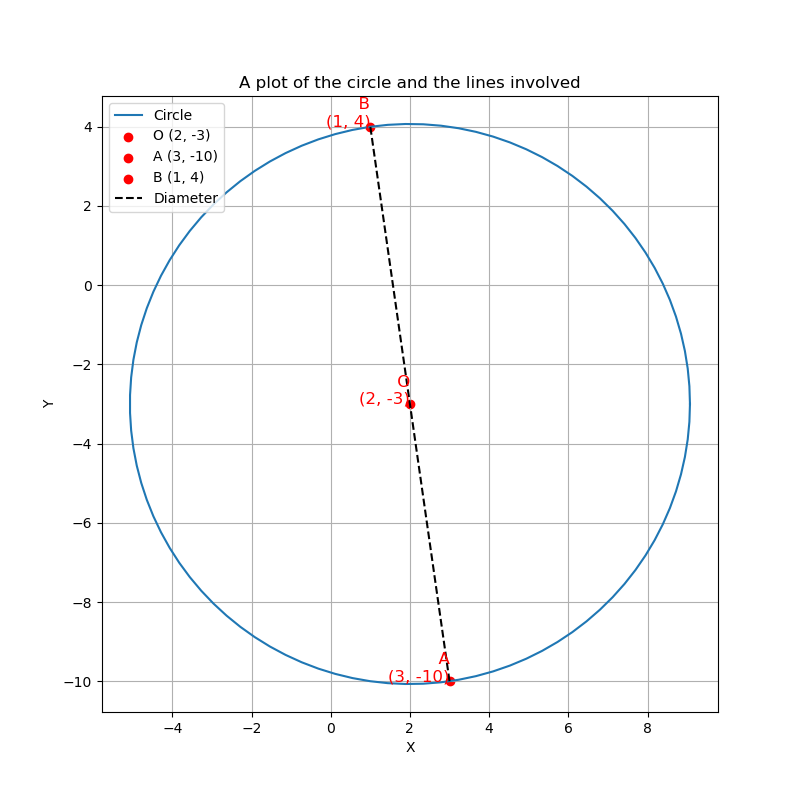
\includegraphics[width=0.75\columnwidth]{figures/Figure.png}
	\caption{A plot of the circle and points invloved}
	\label{fig}
\end{figure}

Code for plotting points and circle
\begin{lstlisting}
	codes/code.py
\end{lstlisting}

\renewcommand{\thefigure}{\theenumi}
\renewcommand{\thetable}{\theenumi}


\end{document}
